\section{The Neuron}

In 1873, an Italian scientist named \textit{\textbf{Camillo Golgi}} discovered a silver staining technique that revealed something extraordinary: the fine cellular architecture of the brain. In 1890, a Spanish neuroscientist and artist, \textit{\textbf{Santiago Ramón y Cajal}} took Golgi's stain and produced breathtaking drawings that showed brain as connected architecture of individual, separate units --- not a continuous mesh as many thought. Cajal proposed what we now call the \textit{Neuron Doctrine}: that the brain is made up of individual units, now known as \textbf{neurons}, that communicate across small gaps by transmitting chemicals (signals), which we now call \textbf{synapses}. 

The exact working of the brain was little understood by the 1940s. However, one thing was known: neurons form a network, and based on the signals they receive from other neurons, they decide whether to release a signal themselves, a process called \textit{firing}, or not. Enter \textit{\textbf{Warren McCulloch}}, a neurophysiologist, and \textit{\textbf{Walter Pitts}}, a brilliant young logician who had taught himself formal logic as a teenager. In 1943, in a small research lab in Chicago, they published a revolutionary paper: \textit{A Logical Calculus of the Ideas Immanent in Nervous Activity} \cite{mcculloch_pitts}. 

In their paper they proposed that each neuron functions as a binary threshold unit. Neurons receive multiple input signals, aggregate them, and produce an output (i.e., \textit{fire}) only if the aggregated signal crosses a certain threshold. Formally, the \textbf{McCulloch-Pitts model} defines a neuron that receives inputs $\mathbf{x} = (x_1,\text{ }x_2,\text{ } \dots, \text{ }x_n)$, where any input $x_i \in \{0, 1\}$. The neuron aggregates the inputs by computing the sum $g(\mathbf{x}) = \sum_{i=1}^{n} x_i$. 

The output is then determined by a fixed constant known as the \textit{thresholding parameter}, $\theta$, as
$$
y = f(g(\mathbf{x})) = 
\begin{cases}
1 & \text{if } g(\mathbf{x}) \geq \theta \\
0 & \text{if } g(\mathbf{x}) < \theta
\end{cases}
$$

Geometrically, a single McCulloch-Pitts neuron divides the space of input points into two regions by a decision boundary defined by the equation $\sum_{i=1}^n x_i - \theta = 0$. For the case of two binary inputs, this line partitions the four possible input points into two groups: those for which $\sum x_i < \theta$ (which produce output 0) and those for which $\sum x_i \geq \theta$ (which produce output 1). Thus, the decision boundary acts as a separator in the input space.

This idea naturally extends to higher dimensions. If the neuron receives three inputs, the line becomes a plane: $\sum_{i=1}^3 x_i - \theta = 0$. For instance, in the case of the 3-input OR function, the desired plane must separate the point (0,0,0) which should produce output 0, from the other seven binary combinations, which should all produce output 1.

\begin{figure}[h]
    \centering
    \subfloat[AND Gate]{
        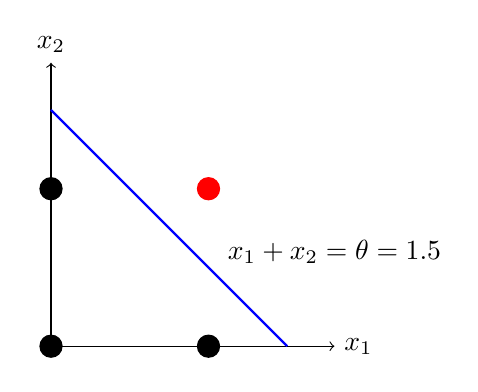
\begin{tikzpicture}[scale=2]
            \draw[->] (0,0) -- (1.8,0) node[right] {$x_1$};
            \draw[->] (0,0) -- (0,1.8) node[above] {$x_2$};

            \filldraw[black] (0,0) circle (2pt);
            \filldraw[black] (1,0) circle (2pt);
            \filldraw[black] (0,1) circle (2pt);
            \filldraw[red] (1,1) circle (2pt);

            \draw[thick, blue] (0,1.5) -- (1.5,0);
            \node at (1.8,0.6) [black] {$x_1 + x_2 = \theta = 1.5$};
        \end{tikzpicture}
    }
    \hspace{80pt}
    \subfloat[OR Gate]{
        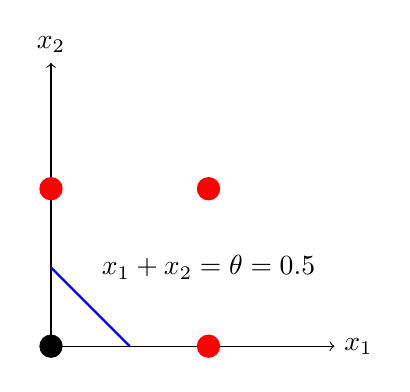
\begin{tikzpicture}[scale=2]
            \draw[->] (0,0) -- (1.8,0) node[right] {$x_1$};
            \draw[->] (0,0) -- (0,1.8) node[above] {$x_2$};

            \filldraw[black] (0,0) circle (2pt);
            \filldraw[red] (1,0) circle (2pt);
            \filldraw[red] (0,1) circle (2pt);
            \filldraw[red] (1,1) circle (2pt);

            \draw[thick, blue] (0,0.5) -- (0.5,0);
            \node at (1,0.5) [black] {$x_1 + x_2 = \theta = 0.5$};
        \end{tikzpicture}
    }
    \caption{McCulloch-Pitts neuron implementing logical functions via thresholding}
\end{figure}

The McCulloch-Pitts neuron provides a foundational abstraction of a biological neuron, but it also raises several important questions. \textit{What if the inputs are not binary but real-valued? Do we always need to manually specify the threshold parameter? Are all inputs equally important, or should some be assigned more weight?} Finally, \textit{can such a neuron model functions that are not linearly separable?}
